\documentclass[]{article}
\usepackage{lmodern}
\usepackage{amssymb,amsmath}
\usepackage{ifxetex,ifluatex}
\usepackage{fixltx2e} % provides \textsubscript
\ifnum 0\ifxetex 1\fi\ifluatex 1\fi=0 % if pdftex
  \usepackage[T1]{fontenc}
  \usepackage[utf8]{inputenc}
\else % if luatex or xelatex
  \ifxetex
    \usepackage{mathspec}
  \else
    \usepackage{fontspec}
  \fi
  \defaultfontfeatures{Ligatures=TeX,Scale=MatchLowercase}
\fi
% use upquote if available, for straight quotes in verbatim environments
\IfFileExists{upquote.sty}{\usepackage{upquote}}{}
% use microtype if available
\IfFileExists{microtype.sty}{%
\usepackage{microtype}
\UseMicrotypeSet[protrusion]{basicmath} % disable protrusion for tt fonts
}{}
\usepackage[margin=1in]{geometry}
\usepackage{hyperref}
\hypersetup{unicode=true,
            pdftitle={Transport-Reachability-Network Analysis},
            pdfauthor={Johannes Bubeck},
            pdfborder={0 0 0},
            breaklinks=true}
\urlstyle{same}  % don't use monospace font for urls
\usepackage{color}
\usepackage{fancyvrb}
\newcommand{\VerbBar}{|}
\newcommand{\VERB}{\Verb[commandchars=\\\{\}]}
\DefineVerbatimEnvironment{Highlighting}{Verbatim}{commandchars=\\\{\}}
% Add ',fontsize=\small' for more characters per line
\usepackage{framed}
\definecolor{shadecolor}{RGB}{248,248,248}
\newenvironment{Shaded}{\begin{snugshade}}{\end{snugshade}}
\newcommand{\AlertTok}[1]{\textcolor[rgb]{0.94,0.16,0.16}{#1}}
\newcommand{\AnnotationTok}[1]{\textcolor[rgb]{0.56,0.35,0.01}{\textbf{\textit{#1}}}}
\newcommand{\AttributeTok}[1]{\textcolor[rgb]{0.77,0.63,0.00}{#1}}
\newcommand{\BaseNTok}[1]{\textcolor[rgb]{0.00,0.00,0.81}{#1}}
\newcommand{\BuiltInTok}[1]{#1}
\newcommand{\CharTok}[1]{\textcolor[rgb]{0.31,0.60,0.02}{#1}}
\newcommand{\CommentTok}[1]{\textcolor[rgb]{0.56,0.35,0.01}{\textit{#1}}}
\newcommand{\CommentVarTok}[1]{\textcolor[rgb]{0.56,0.35,0.01}{\textbf{\textit{#1}}}}
\newcommand{\ConstantTok}[1]{\textcolor[rgb]{0.00,0.00,0.00}{#1}}
\newcommand{\ControlFlowTok}[1]{\textcolor[rgb]{0.13,0.29,0.53}{\textbf{#1}}}
\newcommand{\DataTypeTok}[1]{\textcolor[rgb]{0.13,0.29,0.53}{#1}}
\newcommand{\DecValTok}[1]{\textcolor[rgb]{0.00,0.00,0.81}{#1}}
\newcommand{\DocumentationTok}[1]{\textcolor[rgb]{0.56,0.35,0.01}{\textbf{\textit{#1}}}}
\newcommand{\ErrorTok}[1]{\textcolor[rgb]{0.64,0.00,0.00}{\textbf{#1}}}
\newcommand{\ExtensionTok}[1]{#1}
\newcommand{\FloatTok}[1]{\textcolor[rgb]{0.00,0.00,0.81}{#1}}
\newcommand{\FunctionTok}[1]{\textcolor[rgb]{0.00,0.00,0.00}{#1}}
\newcommand{\ImportTok}[1]{#1}
\newcommand{\InformationTok}[1]{\textcolor[rgb]{0.56,0.35,0.01}{\textbf{\textit{#1}}}}
\newcommand{\KeywordTok}[1]{\textcolor[rgb]{0.13,0.29,0.53}{\textbf{#1}}}
\newcommand{\NormalTok}[1]{#1}
\newcommand{\OperatorTok}[1]{\textcolor[rgb]{0.81,0.36,0.00}{\textbf{#1}}}
\newcommand{\OtherTok}[1]{\textcolor[rgb]{0.56,0.35,0.01}{#1}}
\newcommand{\PreprocessorTok}[1]{\textcolor[rgb]{0.56,0.35,0.01}{\textit{#1}}}
\newcommand{\RegionMarkerTok}[1]{#1}
\newcommand{\SpecialCharTok}[1]{\textcolor[rgb]{0.00,0.00,0.00}{#1}}
\newcommand{\SpecialStringTok}[1]{\textcolor[rgb]{0.31,0.60,0.02}{#1}}
\newcommand{\StringTok}[1]{\textcolor[rgb]{0.31,0.60,0.02}{#1}}
\newcommand{\VariableTok}[1]{\textcolor[rgb]{0.00,0.00,0.00}{#1}}
\newcommand{\VerbatimStringTok}[1]{\textcolor[rgb]{0.31,0.60,0.02}{#1}}
\newcommand{\WarningTok}[1]{\textcolor[rgb]{0.56,0.35,0.01}{\textbf{\textit{#1}}}}
\usepackage{graphicx,grffile}
\makeatletter
\def\maxwidth{\ifdim\Gin@nat@width>\linewidth\linewidth\else\Gin@nat@width\fi}
\def\maxheight{\ifdim\Gin@nat@height>\textheight\textheight\else\Gin@nat@height\fi}
\makeatother
% Scale images if necessary, so that they will not overflow the page
% margins by default, and it is still possible to overwrite the defaults
% using explicit options in \includegraphics[width, height, ...]{}
\setkeys{Gin}{width=\maxwidth,height=\maxheight,keepaspectratio}
\IfFileExists{parskip.sty}{%
\usepackage{parskip}
}{% else
\setlength{\parindent}{0pt}
\setlength{\parskip}{6pt plus 2pt minus 1pt}
}
\setlength{\emergencystretch}{3em}  % prevent overfull lines
\providecommand{\tightlist}{%
  \setlength{\itemsep}{0pt}\setlength{\parskip}{0pt}}
\setcounter{secnumdepth}{5}
% Redefines (sub)paragraphs to behave more like sections
\ifx\paragraph\undefined\else
\let\oldparagraph\paragraph
\renewcommand{\paragraph}[1]{\oldparagraph{#1}\mbox{}}
\fi
\ifx\subparagraph\undefined\else
\let\oldsubparagraph\subparagraph
\renewcommand{\subparagraph}[1]{\oldsubparagraph{#1}\mbox{}}
\fi

%%% Use protect on footnotes to avoid problems with footnotes in titles
\let\rmarkdownfootnote\footnote%
\def\footnote{\protect\rmarkdownfootnote}

%%% Change title format to be more compact
\usepackage{titling}

% Create subtitle command for use in maketitle
\providecommand{\subtitle}[1]{
  \posttitle{
    \begin{center}\large#1\end{center}
    }
}

\setlength{\droptitle}{-2em}

  \title{Transport-Reachability-Network Analysis}
    \pretitle{\vspace{\droptitle}\centering\huge}
  \posttitle{\par}
  \subtitle{Assignment im Rahmen der Vorlesung `Social Network Analyis'}
  \author{Johannes Bubeck}
    \preauthor{\centering\large\emph}
  \postauthor{\par}
    \date{}
    \predate{}\postdate{}
  
\usepackage{graphicx} \usepackage{fancyhdr}

\pagestyle{fancy} \setlength\headheight{28pt}
\fancyhead[L]{
\includegraphics[width=2.5cm]{Data/logo.png}}
\fancyfoot[LE,RO]{GPIM}

\begin{document}
\maketitle

{
\setcounter{tocdepth}{2}
\tableofcontents
}
\hypertarget{einleitung}{%
\section{Einleitung}\label{einleitung}}

\hypertarget{vorgehensweise-und-zielsetzung}{%
\subsection{Vorgehensweise und
Zielsetzung}\label{vorgehensweise-und-zielsetzung}}

Die Zielsetzung dieses Projekts ist die Durchführung einer ``Social
Network Analysis'' im Rahmen der Leistungsbeurteilung des gleichnamigen
DHBW-Kurses. Die Datenbasis der Analyse und des Assignments stellt der
Datensatz ``Airline travel reachability network'' dar
(\url{https://snap.stanford.edu/data/reachability.html}).

Folgende Abbildung zeigt die Vorgehensweise dieses Projekts. In der
Einleitung wird das Vorgehen des ``Social Network Analysis Projekts''
beschrieben. Weiterhin wird die Zielsetzung und die des Assignment
zugrundeliegende Forschungsfrage definiert. Der Hauptteil des
Assignments bildet eine ``klassische'' Vorgehensweise im Data Analytics
Bereich ab. In einem ersten Schritt wird zunächst der theoretische
Hintergrund des Projekts dargelegt. Dazu werden unter anderem Punkte wie
die verfügbaren Daten, die Netzwerkdefinition, Flow Struktur und das
Zentralitätsmaß näher beleichtet. Nach der Datenvorverarbeitung und dem
Laden der notwendigen Bibliotheken, die für die Analyse notwendig sind,
erfolgt der Datenimport. Weiterhin dient eine Explorative Analyse der
Daten näheren Einblicken in die verfügbaren Daten und deren Qualität.
Schließlich wird im letzten Schritt des Hauptteils die Modellierung und
Visualisierung durchgeführt. Das Fazit beschäftigt sich zum Einen mit
der Bündelung und Präsentation der Daten und zum Anderen einem Ausblick.

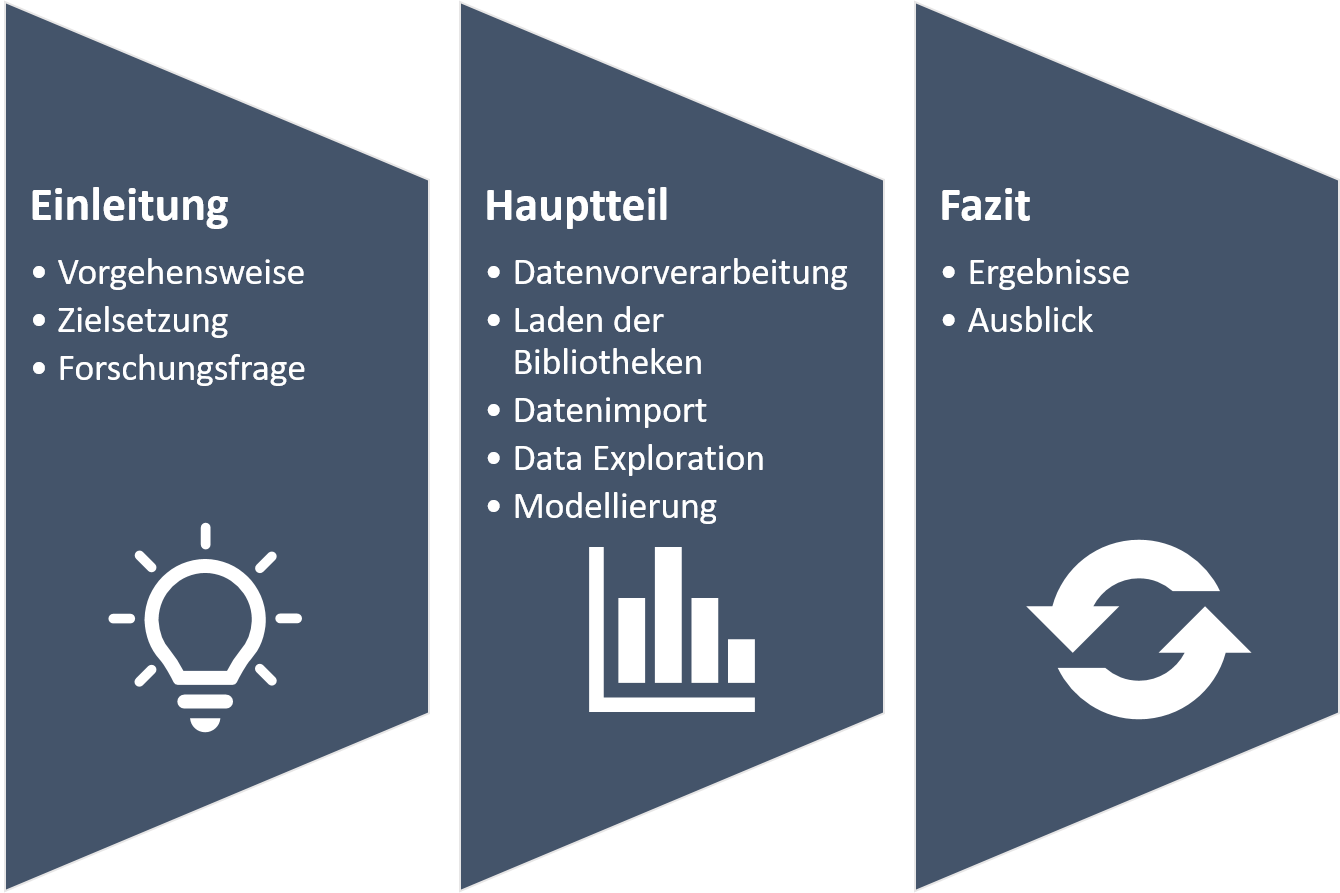
\includegraphics[width=0.5\textwidth,height=\textheight]{Data/Vorgehensweise.png}

\hypertarget{forschungsfrage}{%
\subsection{Forschungsfrage}\label{forschungsfrage}}

Der Datensatz ``Airline travel reachability network'' bildet
Flugverbindungen für Flughäfen in den Vereinigten Staaten sowie Kanada
ab. Zusätzlich sind dem Datensatz Informationen zu den Einwohnern der
jeweiligen Stadt sowie geometrischen Daten in Form von Längen- und
Breitengraden. Mit diesen Informationen bietet sich folgende
Forschungsfrage an:

Werden Flughäfen in Städten mit mehr Einwohnern häufiger angeflogen, als
Städte mit weniger Population?

\hypertarget{hauptteil}{%
\section{Hauptteil}\label{hauptteil}}

\hypertarget{theoretischer-hintergrund}{%
\subsection{Theoretischer Hintergrund}\label{theoretischer-hintergrund}}

Das Kapitel theoretischer Hintergrund dient dem Verständnis der
nachfolgenden Netzwerkanalyse. Es wird unter anderem auf den Datensatz
an sich eingegangen, der Netzwerktyp analysiert und Flow Struktur und
Zentralitätsmaße erörtert.

\hypertarget{datensatz}{%
\subsubsection{Datensatz}\label{datensatz}}

Bei dem Datensatz ``Airline travel reachability network'' handelt es
sich um ein Netzwerk für die Erreichbarkeit von Städten in den
Vereinigten Staaten und Kanada. Die Knoten im Datensatz bilden die
einzelnen Flughäfen der Städte. Die Kanten repräsentieren die
Flugverbindung. Diese sind so gewichtet, dass es eine Kante von Stadt i
zu Stadt j gibt, wenn die geschätzte Flugreisezeit unter einem
Schwellenwert liegt. Die Reisezeit schließt geschätzte Verspätungen bei
Zwischenlandungen mit ein. Zusätzlich beinhalet der Datensatz, wie
bereits erwähnt, Informationen zu den Einwohnern der jeweiligen Stadt
sowie geometrischen Daten in Form von Längen- und Breitengraden.

\hypertarget{netzwerkdefinition}{%
\subsubsection{Netzwerkdefinition}\label{netzwerkdefinition}}

Die Definition des Netzwerktyps beschreibt zum Einen WIE die Daten
erhoben worden sind und zum Anderen aber auch WELCHE und WIEVIELE
Datenpunkte zur Verfügung stehen. Bei dem zugrundeliegenden Datensatz
ist der Ursprung der Erhebung nicht publiziert. Daher lässt sich die
Frage ob es sich bei der Erhebung um ``Custom-made'' Daten oder
``Ready-made'' Daten handelt nur in der Theorie beantworten. Sollte es
sich um Custom-made Daten handeln wurden diese für einen spezifischen
Zweck hin gesammelt. Dies kann durch Umfragen, Schneeball Analysen oder
mithilfe einer Gesamterhebung stattfinden.

Bei Ready-made Daten ist der Datensatz als Nebenprodukt entstanden. Bei
diesem Netzwerk ist es denkbar, dass mithilfe von Web-Crawlern
bestimmter APIs die Daten abgezogen worden sind, beispielsweise von
Buchungsseiten für Flugverbindungen oder ``Arrival-Departure'' Seiten.

Weiterhin kann ein Netzwerk über einen Grundtyp definiert werden.
Hierbei gibt es einerseits das Ego-Netzwerk, bei dem Beziehnungen eines
Akeurs (Ego) zu anderen Akteuren (Alteri) der direkten Netzwerkumgebung,
sowie den Beziehungen zwischen den Akteuren analysiert werden. Als
zweite Möglichkeit gibt es Schneeball-Netzwerke oder auch referentielles
Netzwerk genannt. Hierbei wird mit einem Sample durch eine Erhebung
gestartet und dann jeder Akteur zu den Attributdaten befragt. Die
Erhebung endet wenn das Netzwerk gesättigt ist. Die Gesamterhebung
analysiert alle Elemente eines Netzwerks inklusive deren Attribute und
Beziehungen untereinander.

Bei dem ``Airline travel reachability network'' handelt es sich
wahrscheinlich um eine Gesamterhebung aller Flugverbindungen.

\hypertarget{zentralituxe4tsmauxdf}{%
\subsubsection{Zentralitätsmaß}\label{zentralituxe4tsmauxdf}}

Um ein Netzwerk beziehungsweise einen Graphen analysieren zu können, ist
die Wichtigkeit der Knoten und deren Kanten von hoher Bedeutung. Für die
Analyse und die Beantwortung der Forschungsfrage ist die Anwendung von
sogenannten Zentralitätsmaßen essentiell.

Die Forschungsfrage ``Werden Flughäfen in Städten mit mehr Einwohnern
häufiger angeflogen, als Städte mit weniger Population?'' wird in zwei
Schritten beantwortet. Mithilfe des Zentralitätsmaßes ``degree
centrality'' kann der Knoten mit der höchsten Zentralität im Netzwerk
gefunden werden. Dies entspricht der Stadt beziehungsweise Flughafen mit
den meisten Kanten, also den meisten Flugverbindungen. Anschließend kann
geprüft werden, ob dieser Flughafen auch eine hohe Population hat.

\hypertarget{datenvorverarbeitung}{%
\subsection{Datenvorverarbeitung}\label{datenvorverarbeitung}}

\hypertarget{laden-der-bibliotheken}{%
\subsubsection{Laden der Bibliotheken}\label{laden-der-bibliotheken}}

Als ersten Schritt der Datenvorverarbeitung werden die benötigten
Bibliotheken für das Data-Wrangling, DIe Modellierung sowie die
Visualisierungen geladen.

\begin{Shaded}
\begin{Highlighting}[]
\KeywordTok{library}\NormalTok{(}\StringTok{"tidyverse"}\NormalTok{)}
\KeywordTok{library}\NormalTok{(}\StringTok{"igraph"}\NormalTok{) }
\KeywordTok{library}\NormalTok{(}\StringTok{"tidygraph"}\NormalTok{) }
\KeywordTok{library}\NormalTok{(}\StringTok{"ggraph"}\NormalTok{)}
\KeywordTok{library}\NormalTok{(}\StringTok{"ggplot2"}\NormalTok{)}
\KeywordTok{library}\NormalTok{(}\StringTok{"tinytex"}\NormalTok{)}
\end{Highlighting}
\end{Shaded}

\hypertarget{datenimport}{%
\subsubsection{Datenimport}\label{datenimport}}

Die Datenbasis für das Projekt besteht aus zwei CSV-Dateien, welche
mithilfe eines Imports aus dem Ordner ``Data'' in das Environment
geladen werden können. Im Datensatz ``Dat'' befinden sich neben der
node\_id alle relevanten Zusatzinformationen wie die Geo-Daten, die
Bevölkerung sowie die vollständigen Namen der Städte des Flughafens.
``Dat2'' beinhaltet zum eine ID-Spalte sowie alle Flugverbindungen als
Kantenliste.

\begin{Shaded}
\begin{Highlighting}[]
\NormalTok{dat <-}\StringTok{ }\KeywordTok{read_csv}\NormalTok{(}\StringTok{'Data/reachability-meta.csv'}\NormalTok{)}
\NormalTok{dat2 <-}\StringTok{ }\KeywordTok{read.table}\NormalTok{(}\StringTok{'Data/reachability.txt'}\NormalTok{)}
\end{Highlighting}
\end{Shaded}

Nach erfolgreichem Datenimport und Betrachtung der Daten sind zwei
Schritte nötig: Zum Einen müssen die Spalten des Datensatzes ``dat2''
umbenannt werden und zum Anderen negative Werte in positive umgewandelt
werden.

\begin{Shaded}
\begin{Highlighting}[]
\NormalTok{dat2 <-}\StringTok{ }\NormalTok{dat2 }\OperatorTok\StringTok{ }
\StringTok{  }\KeywordTok{rename}\NormalTok{(}
    \DataTypeTok{from =}\NormalTok{ V1,}
    \DataTypeTok{weight =}\NormalTok{ V2,}
    \DataTypeTok{to =}\NormalTok{ V3}
\NormalTok{  )}
\end{Highlighting}
\end{Shaded}

\begin{Shaded}
\begin{Highlighting}[]
\NormalTok{dat2}\OperatorTok{$}\NormalTok{to <-}\StringTok{ }\NormalTok{dat2}\OperatorTok{$}\NormalTok{to}\OperatorTok{*}\NormalTok{(}\OperatorTok{-}\DecValTok{1}\NormalTok{)}
\end{Highlighting}
\end{Shaded}

\hypertarget{daten-exploration}{%
\subsection{Daten Exploration}\label{daten-exploration}}

Die Erkundung der zur Verfügung stehenden Datenbasis findet im Kapitel
``Daten Exploration'' statt. Als ersten Schritt wird jeweils mit dem
Befehl ``head()'' der Kopf des Datensatzes ausgegeben und betrachtet.

Weiterhin kann über ``summary()'' ein Blick auf die Datentypen und erste
Statistiken des Datensatzes geworfen werden. Damit ist es möglich ein
erstes Gefühl für die Datenbasis zu bekommen und eventuelle fehlende
Daten oder falsche Datentypen in einem ``Data-Cleaning'' zu beheben. In
diesem Fall sind neben der Spaltenumbenennung und der Konvertierung der
negativen Werte keine weiteren Manipulationen nötig.

\begin{Shaded}
\begin{Highlighting}[]
\KeywordTok{head}\NormalTok{(dat)}
\end{Highlighting}
\end{Shaded}

\begin{verbatim}
## # A tibble: 6 x 5
##   node_id name             metro_pop latitude longitude
##     <dbl> <chr>                <dbl>    <dbl>     <dbl>
## 1       0 Abbotsford, BC      133497     49.1    -122. 
## 2       1 Aberdeen, SD         40878     45.5     -98.5
## 3       2 Abilene, TX         166416     32.4     -99.7
## 4       3 Akron/Canton, OH    701456     40.8     -81.4
## 5       4 Alamosa, CO           9433     37.5    -106. 
## 6       5 Albany, GA          157688     31.6     -84.2
\end{verbatim}

\begin{Shaded}
\begin{Highlighting}[]
\KeywordTok{summary}\NormalTok{(dat)}
\end{Highlighting}
\end{Shaded}

\begin{verbatim}
##     node_id          name             metro_pop           latitude    
##  Min.   :  0.0   Length:456         Min.   :     538   Min.   :19.64  
##  1st Qu.:113.8   Class :character   1st Qu.:   49513   1st Qu.:35.22  
##  Median :227.5   Mode  :character   Median :  158892   Median :40.79  
##  Mean   :227.5                      Mean   :  713095   Mean   :40.69  
##  3rd Qu.:341.2                      3rd Qu.:  496238   3rd Qu.:45.47  
##  Max.   :455.0                      Max.   :19020000   Max.   :71.29  
##    longitude      
##  Min.   :-165.40  
##  1st Qu.:-110.70  
##  Median : -92.45  
##  Mean   : -96.72  
##  3rd Qu.: -81.24  
##  Max.   : -55.61
\end{verbatim}

\begin{Shaded}
\begin{Highlighting}[]
\KeywordTok{head}\NormalTok{(dat2)}
\end{Highlighting}
\end{Shaded}

\begin{verbatim}
##   from weight   to
## 1   27      0  757
## 2   57      0   84
## 3   70      0 1290
## 4   74      0  465
## 5   86      0  700
## 6   94      0  526
\end{verbatim}

\begin{Shaded}
\begin{Highlighting}[]
\KeywordTok{summary}\NormalTok{(dat2)}
\end{Highlighting}
\end{Shaded}

\begin{verbatim}
##       from           weight            to        
##  Min.   :  0.0   Min.   :  0.0   Min.   :  10.0  
##  1st Qu.:109.0   1st Qu.:107.0   1st Qu.: 217.0  
##  Median :237.0   Median :235.0   Median : 282.0  
##  Mean   :227.3   Mean   :226.4   Mean   : 348.1  
##  3rd Qu.:342.0   3rd Qu.:340.0   3rd Qu.: 397.0  
##  Max.   :455.0   Max.   :455.0   Max.   :2855.0
\end{verbatim}

\hypertarget{modellierung}{%
\subsection{Modellierung}\label{modellierung}}

Ziel des Kapitels Modellierung ist zum Einen ein Netzwerkobjekt als
``tbl\_graph'' zu modellieren und zum Anderen weitere Attribute und
Werte zu berechnen, die für die Visualisierungen und die Beantwortung
der Forschungsfrage im ``Fazit'' notwendig sind.

Durch die Funktion ``as\_tbl\_graph'' kann die Kantenliste ganz einfach
als tbl\_object umgewandelt und als ``net'' gespeichert werden.

\begin{Shaded}
\begin{Highlighting}[]
\NormalTok{net <-}\StringTok{ }\KeywordTok{as_tbl_graph}\NormalTok{(dat2)}
\end{Highlighting}
\end{Shaded}

Der nächste Schritt in der Netzwerkanalyse ist, wie im Kapitel
``Zentralitätsmaße'' erwähnt, die Berechnung des Grad der Zentralität.
Dafür kann mithilfe der Funktion ``degree'' ganz einfach der Grad jedes
Knoten berechnet werden. Um die berechneten Werte später verwenden zu
können, wir das Array zusätzlich noch in einen Data Frame überführt.
Außerdem werden die Zeilen mit den 10 höchsten Werten zur Betrachtung
ausgegeben.

\begin{Shaded}
\begin{Highlighting}[]
\NormalTok{degree <-}\StringTok{ }\KeywordTok{degree}\NormalTok{(net)}

\NormalTok{degree_df <-}\StringTok{ }\KeywordTok{as.data.frame}\NormalTok{(degree)}

\NormalTok{degree_df }\OperatorTok
\StringTok{  }\KeywordTok{top_n}\NormalTok{(}\DecValTok{10}\NormalTok{)}
\end{Highlighting}
\end{Shaded}

\begin{verbatim}
##    degree
## 1     873
## 2     662
## 3     648
## 4     704
## 5     618
## 6     676
## 7     618
## 8     618
## 9     616
## 10    667
\end{verbatim}

Zur Beantwortung der Forschungsfrage sind die Zusatzinformationen aus
dem Datensatz ``dat'' unerlässlich. Aus diesem Grund werden die beiden
Datensätze im nächsten Schritt ``gejoined'', sodass diese in einem
Datensatz vorliegen.

\begin{Shaded}
\begin{Highlighting}[]
\NormalTok{degree_df <-}\StringTok{ }\KeywordTok{rowid_to_column}\NormalTok{(degree_df, }\StringTok{"node_id"}\NormalTok{)}

\NormalTok{degree_pop_df <-}\StringTok{ }\KeywordTok{merge}\NormalTok{(}\DataTypeTok{x=}\NormalTok{degree_df, }\DataTypeTok{y=}\NormalTok{dat, }\DataTypeTok{by=}\StringTok{"node_id"}\NormalTok{)}
\end{Highlighting}
\end{Shaded}

Interssant für die Interpretation der Daten sind die jeweils 10 höchsten
Werte von Population und dem Grad der Zentralität. Aus diesem Grund
werden diese Im nächsten Schritt berechnet und ausgegeben.

\begin{Shaded}
\begin{Highlighting}[]
\NormalTok{calc_top_degree <-}\StringTok{ }\KeywordTok{top_n}\NormalTok{(}\DataTypeTok{x=}\NormalTok{degree_pop_df, }\DataTypeTok{n=}\DecValTok{10}\NormalTok{, }\DataTypeTok{wt=}\NormalTok{degree)}
\NormalTok{calc_top_degree}
\end{Highlighting}
\end{Shaded}

\begin{verbatim}
##    node_id degree                name metro_pop latitude  longitude
## 1       13    873        Amarillo, TX    253823 35.20726 -101.83389
## 2       16    662       Asheville, NC    429017 35.59846  -82.55314
## 3       18    648          Athens, GA    193317 33.95813  -83.37326
## 4       20    704   Atlantic City, NJ    274338 39.36281  -74.42652
## 5       21    618         Augusta, GA    561858 33.47909  -81.97531
## 6       90    676  Corpus Christi, TX    431381 27.79635  -97.40356
## 7      153    618    Grand Rapids, MI    779604 42.96641  -85.67118
## 8      158    618      Greenbrier, WV     35644 37.97558  -80.42690
## 9      163    616 Gulfport/Biloxi, MS    253511 30.41334  -89.07202
## 10     229    667          Laredo, TX    256496 27.53092  -99.50201
\end{verbatim}

\begin{Shaded}
\begin{Highlighting}[]
\NormalTok{calc_top_pop <-}\StringTok{ }\KeywordTok{top_n}\NormalTok{(}\DataTypeTok{x=}\NormalTok{degree_pop_df, }\DataTypeTok{n=}\DecValTok{10}\NormalTok{, }\DataTypeTok{wt=}\NormalTok{metro_pop)}
\NormalTok{calc_top_pop}
\end{Highlighting}
\end{Shaded}

\begin{verbatim}
##    node_id degree                      name metro_pop latitude  longitude
## 1       53    418               Burbank, CA  12940000 34.18147 -118.30812
## 2       74    392               Chicago, IL   9505000 41.88415  -87.63241
## 3       94    543     Dallas/Fort Worth, TX   6527000 32.92222  -97.04090
## 4      178    380               Houston, TX   6087000 29.76045  -95.36978
## 5      243    342            Long Beach, CA  12940000 33.76642 -118.19239
## 6      244    254 Long Island MacArthur, NY   7568000 40.78913  -73.09839
## 7      246    275           Los Angeles, CA  12940000 34.05329 -118.24501
## 8      294     42              New York, NY  19020000 40.71455  -74.00712
## 9      323    295          Philadelphia, PA   5992000 39.95227  -75.16237
## 10     416    187               Toronto, ON   6324000 43.64856  -79.38533
\end{verbatim}

\hypertarget{visualisierung}{%
\subsection{Visualisierung}\label{visualisierung}}

Das Kapitel Visualisierung dient der erweiterten Daten Exploration.
Mithilfe der nachfolgenden Plots können die Daten noch besser verstanden
werden und weitere Erkenntnisse daraus geschlossen werden.

Als ersten Plot wird die Verteilung des Grad der Zentralität für jeden
Knoten ausgegeben. Dadurch kann ein Gesamtüberblick erreicht werden.
Auffällig hierbei ist, dass es relativ viele Knoten gibt, bei denen der
Grad 0 oder sehr klein ist. Interessant ist jedoch auch, dass es Knoten
mit sehr großen Werten jenseits von 500 gibt. Diese könnten interessant
für die Beantwortung der Forschungsfrage sein.

\begin{Shaded}
\begin{Highlighting}[]
\KeywordTok{ggplot}\NormalTok{(}\DataTypeTok{data =}\NormalTok{ degree_df, }\KeywordTok{aes}\NormalTok{(}\DataTypeTok{x =}\NormalTok{ degree)) }\OperatorTok{+}
\StringTok{  }\KeywordTok{geom_bar}\NormalTok{(}\DataTypeTok{size =} \FloatTok{.8}\NormalTok{, }\DataTypeTok{colour=}\StringTok{"#e2001a"}\NormalTok{) }\OperatorTok{+}
\StringTok{  }\KeywordTok{theme_classic}\NormalTok{() }\OperatorTok{+}
\StringTok{  }\KeywordTok{scale_y_log10}\NormalTok{() }\OperatorTok{+}
\StringTok{  }\KeywordTok{ggtitle}\NormalTok{(}\StringTok{"Verteilung Grad der Zentralität"}\NormalTok{)}
\end{Highlighting}
\end{Shaded}

\includegraphics{Data-Exploration_Portfolio_files/figure-latex/count degree-1.pdf}

Weiterhin ist die Verteilung der Populationszahlen ein wichtiger Schritt
im Verständnis des Datensatzes. Dafür kommt als nächste Visualisierung
ein Boxplot zum Einsatz. Dieser zeigt den Durchschnitt der
Bevölkerungszahlen sowie Ausreißer nach oben und unten.

\begin{Shaded}
\begin{Highlighting}[]
\KeywordTok{ggplot}\NormalTok{(}\DataTypeTok{data =}\NormalTok{ degree_pop_df, }\KeywordTok{aes}\NormalTok{(}\DataTypeTok{y=}\NormalTok{metro_pop)) }\OperatorTok{+}
\StringTok{  }\KeywordTok{geom_boxplot}\NormalTok{(}\DataTypeTok{size =} \FloatTok{.8}\NormalTok{) }\OperatorTok{+}
\StringTok{  }\KeywordTok{theme_classic}\NormalTok{() }\OperatorTok{+}
\StringTok{  }\KeywordTok{scale_y_log10}\NormalTok{() }\OperatorTok{+}
\StringTok{  }\KeywordTok{ggtitle}\NormalTok{(}\StringTok{"Verteilung Bevölkerung"}\NormalTok{)}
\end{Highlighting}
\end{Shaded}

\includegraphics{Data-Exploration_Portfolio_files/figure-latex/pop viz-1.pdf}

Für die Visualisierung des Netzwerks wird aus Übersichtsgründen als
ersten Schritt ein Sample von 200 Datenpunkten extrahiert. Anschließend
folgen drei verschiedene Plots des Netzwerks.

\begin{Shaded}
\begin{Highlighting}[]
\NormalTok{dat_sample <-}\StringTok{ }\KeywordTok{sample_n}\NormalTok{(dat2, }\DecValTok{200}\NormalTok{)}

\NormalTok{net_sample <-}\StringTok{ }\KeywordTok{as_tbl_graph}\NormalTok{(dat_sample)}

\KeywordTok{ggraph}\NormalTok{(net_sample, }\DataTypeTok{layout =} \StringTok{'fr'}\NormalTok{, }\DataTypeTok{maxiter =} \DecValTok{100}\NormalTok{) }\OperatorTok{+}\StringTok{ }
\StringTok{  }\KeywordTok{geom_node_point}\NormalTok{(}\DataTypeTok{colour=}\StringTok{"#e2001a"}\NormalTok{) }\OperatorTok{+}\StringTok{ }
\StringTok{  }\KeywordTok{geom_edge_link}\NormalTok{(}\DataTypeTok{alpha =} \FloatTok{.4}\NormalTok{) }\OperatorTok{+}
\StringTok{  }\KeywordTok{theme_graph}\NormalTok{()}
\end{Highlighting}
\end{Shaded}

\includegraphics{Data-Exploration_Portfolio_files/figure-latex/sample-1.pdf}

\begin{Shaded}
\begin{Highlighting}[]
\KeywordTok{ggraph}\NormalTok{(net_sample, }\DataTypeTok{layout =} \StringTok{'kk'}\NormalTok{, }\DataTypeTok{maxiter =} \DecValTok{100}\NormalTok{) }\OperatorTok{+}\StringTok{ }
\StringTok{  }\KeywordTok{geom_node_point}\NormalTok{(}\DataTypeTok{colour=}\StringTok{"#e2001a"}\NormalTok{) }\OperatorTok{+}\StringTok{ }
\StringTok{  }\KeywordTok{geom_edge_link}\NormalTok{(}\DataTypeTok{alpha =} \FloatTok{.4}\NormalTok{) }\OperatorTok{+}
\StringTok{  }\KeywordTok{theme_graph}\NormalTok{()}
\end{Highlighting}
\end{Shaded}

\begin{verbatim}
## Warning: Removed 2 rows containing non-finite values (stat_edge_link).
\end{verbatim}

\begin{verbatim}
## Warning: Removed 1 rows containing missing values (geom_point).
\end{verbatim}

\includegraphics{Data-Exploration_Portfolio_files/figure-latex/sample-2.pdf}

\begin{Shaded}
\begin{Highlighting}[]
\CommentTok{# coord diagramm}
\KeywordTok{ggraph}\NormalTok{(net_sample, }\DataTypeTok{layout =} \StringTok{'linear'}\NormalTok{, }\DataTypeTok{circular =} \OtherTok{TRUE}\NormalTok{) }\OperatorTok{+}\StringTok{ }
\StringTok{  }\KeywordTok{geom_node_point}\NormalTok{(}\DataTypeTok{colour=}\StringTok{"#e2001a"}\NormalTok{) }\OperatorTok{+}
\StringTok{  }\KeywordTok{geom_edge_arc}\NormalTok{(}\DataTypeTok{alpha =} \FloatTok{.4}\NormalTok{) }\OperatorTok{+}
\StringTok{  }\KeywordTok{theme_graph}\NormalTok{()}
\end{Highlighting}
\end{Shaded}

\includegraphics{Data-Exploration_Portfolio_files/figure-latex/sample-3.pdf}

\hypertarget{fazit}{%
\section{Fazit}\label{fazit}}

\hypertarget{ergebnisse}{%
\subsection{Ergebnisse}\label{ergebnisse}}

\begin{Shaded}
\begin{Highlighting}[]
\NormalTok{max_population <-}\StringTok{ }\KeywordTok{max}\NormalTok{(degree_pop_df}\OperatorTok{$}\NormalTok{metro_pop)}
\NormalTok{min_population <-}\StringTok{ }\KeywordTok{min}\NormalTok{(degree_pop_df}\OperatorTok{$}\NormalTok{metro_pop)}
\NormalTok{mean_population <-}\StringTok{ }\KeywordTok{mean}\NormalTok{(degree_pop_df}\OperatorTok{$}\NormalTok{metro_pop)}

\NormalTok{mean_population_df <-}\StringTok{ }\KeywordTok{data.frame}\NormalTok{(mean_population)}


\NormalTok{calc_top_degree}\OperatorTok{$}\NormalTok{mean_population <-}\StringTok{ }\NormalTok{mean_population}
\end{Highlighting}
\end{Shaded}

\begin{Shaded}
\begin{Highlighting}[]
\KeywordTok{ggplot}\NormalTok{(calc_top_degree, }\KeywordTok{aes}\NormalTok{(}\DataTypeTok{x=}\NormalTok{name, }\DataTypeTok{y=}\NormalTok{metro_pop))}\OperatorTok{+}
\StringTok{  }\KeywordTok{geom_col}\NormalTok{(}\DataTypeTok{size=}\DecValTok{5}\NormalTok{, }\DataTypeTok{alpha=}\NormalTok{.}\DecValTok{7}\NormalTok{) }\OperatorTok{+}
\StringTok{  }\KeywordTok{scale_y_continuous}\NormalTok{(}\DataTypeTok{labels =}\NormalTok{ scales}\OperatorTok{::}\NormalTok{comma) }\OperatorTok{+}
\StringTok{  }\KeywordTok{geom_hline}\NormalTok{(}\DataTypeTok{yintercept=}\NormalTok{mean_population, }\DataTypeTok{colour =} \StringTok{"#e2001a"}\NormalTok{, }\DataTypeTok{linetype=}\StringTok{"dashed"}\NormalTok{) }\OperatorTok{+}
\StringTok{  }\KeywordTok{geom_text}\NormalTok{(}\KeywordTok{aes}\NormalTok{(}\DecValTok{0}\NormalTok{,}\KeywordTok{round}\NormalTok{(mean_population, }\DataTypeTok{digits =} \DecValTok{0}\NormalTok{), }\DataTypeTok{label =} \KeywordTok{round}\NormalTok{(mean_population, }\DataTypeTok{digits =} \DecValTok{0}\NormalTok{), }\DataTypeTok{vjust =} \DecValTok{-1}\NormalTok{, }\DataTypeTok{hjust =} \FloatTok{-.5}\NormalTok{), }\DataTypeTok{colour =} \StringTok{"#e2001a"}\NormalTok{) }\OperatorTok{+}
\StringTok{  }\KeywordTok{theme_minimal}\NormalTok{() }\OperatorTok{+}
\StringTok{  }\KeywordTok{theme}\NormalTok{(}\DataTypeTok{axis.text.x =} \KeywordTok{element_text}\NormalTok{(}\DataTypeTok{angle =} \DecValTok{45}\NormalTok{, }\DataTypeTok{vjust =} \FloatTok{0.5}\NormalTok{, }\DataTypeTok{hjust=}\DecValTok{1}\NormalTok{)) }\OperatorTok{+}
\StringTok{  }\KeywordTok{xlab}\NormalTok{(}\StringTok{""}\NormalTok{) }\OperatorTok{+}
\StringTok{  }\KeywordTok{ylab}\NormalTok{(}\StringTok{"Population"}\NormalTok{) }\OperatorTok{+}
\StringTok{  }\KeywordTok{ggtitle}\NormalTok{(}\StringTok{"Top 10 - Grad der Zentralität und Bevölkerung"}\NormalTok{)}
\end{Highlighting}
\end{Shaded}

\includegraphics{Data-Exploration_Portfolio_files/figure-latex/results-1.pdf}

\hypertarget{reflexion}{%
\subsection{Reflexion}\label{reflexion}}


\end{document}
